\section{Introduction}

\noindent\hspace*{\parindent} Start your introduction here. Explain the background of your problem, why it matters, and what gap in existing work your thesis addresses.

\subsection{Background}
\noindent\hspace*{\parindent} Describe the context and prior work related to your topic. Cite sources using \texttt{\textbackslash cite\{\}}, for example \cite{williams2017information}.

\subsection{Problem Statement}
\noindent\hspace*{\parindent} State clearly what problem your thesis solves.

\subsection{Objectives}
\noindent\hspace*{\parindent} List the objectives of your research, e.g. using an itemized list:
\begin{itemize}
    \item First objective.
    \item Second objective.
    \item Third objective.
\end{itemize}

\subsection{Thesis Structure}
\noindent\hspace*{\parindent} Briefly outline how the rest of the thesis is organized (one sentence per chapter/section is typical).

\begin{figure}[H]
    \centering
    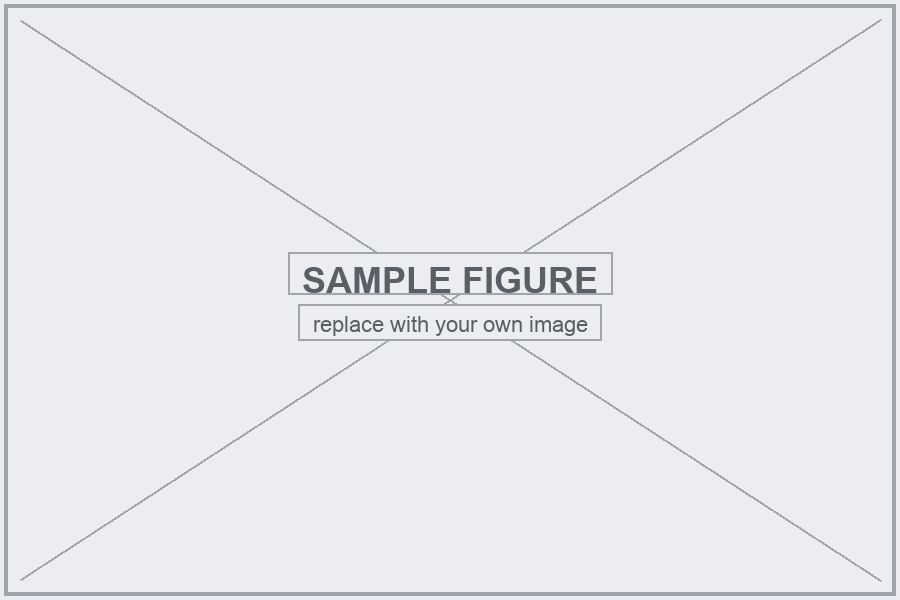
\includegraphics[width=0.6\textwidth]{figure/sample-figure.png}
    \caption{Example figure -- replace with a diagram of your own, e.g. an overview of your thesis concept}
    \label{fig:intro-overview}
\end{figure}
